\subsection{Serverseitig}
\subsubsection{RemoteLogger}
\label{sec:RemoteLogger}
\begin{wrapfigure}[14]{r}[0cm]{205px}
	\vspace{-10px} \hspace{5px}
	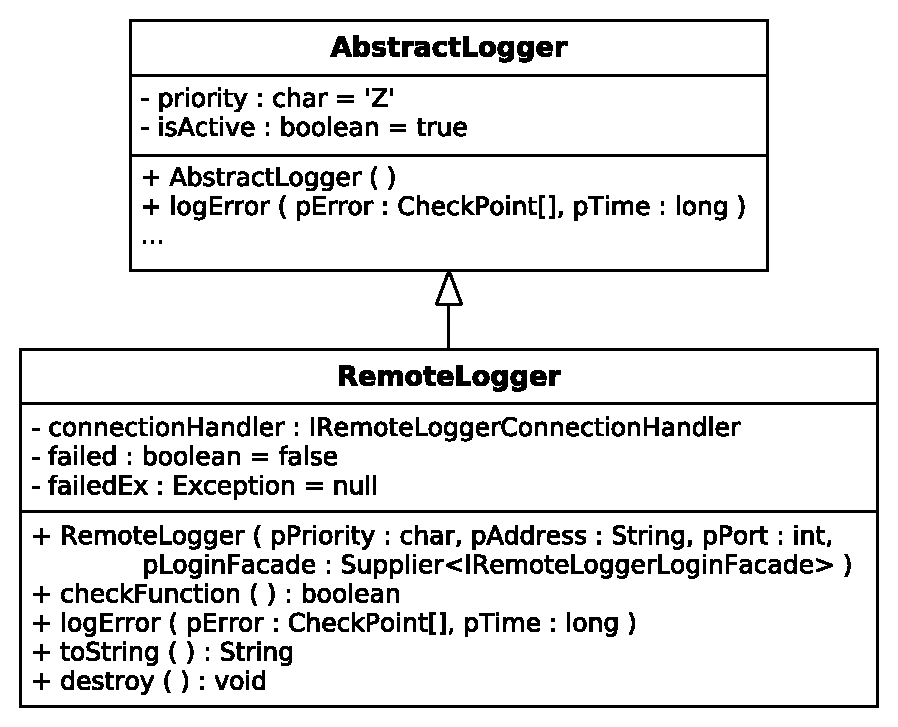
\includegraphics[width=200px]{../img/CD-RemoteLogger.eps}
	\caption{Aufbau des \glqq RemoteLogger\grqq}
\end{wrapfigure}
\par Diese Klasse wird im bisher vorhandenen Logging-Modul von ADITO4 registriert und dient als Einstiegspunkt des Remote-Loggings. Über den Konstruktor wird die Priorität des Logger bestimmt. Diese besagt, ab welcher Dringlichkeitsstufe Meldungen geloggt werden dürfen. Ebenso werden hier Hostadresse und Hostport zugewiesen. Um später die eingehenden Login-Anfragen der Remote-Logger-Clients annehmen/ablehnen zu können, benötigt man zusätzlich eine \glqq IRemoteLoggerLoginFacade\grqq\ (siehe \prettyref{sec:IRemoteLoggerLoginFacade}), die ebenso im Konstruktor ihren Platz findet.
\par Der Remote-Logger erbt von der abstrakten Klasse \glqq AbstractLogger\grqq\ wodurch es möglich ist, mit der Methode \glqq logError(...)\grqq\ auf vom System übergebene CheckPoint-Arrays zu reagieren. Diese übergebenen Arrays sind jedoch noch nicht serialisierbar und können somit nicht über das Netzwerk geschickt werden. Eine Kapselung der Meldung in ein serialisierbares Objekt ist hier notwendig. Ebenso soll es möglich sein, die Meldung eines CheckPoints abhängig von der verbindungsspezifischen Sprache zu übersetzen. Hierzu dient das Interface \glqq IRemoteLoggerCheckPoint\grqq\ und ihre Implementierung \glqq TranslateableRemoteLoggerCheckPoint\grqq\ (siehe \prettyref{sec:IRemoteLoggerCheckPoint}).
\par Sobald die Umwandlung der CheckPoints abgeschlossen ist, werden diese dem \glqq connectionHandler\grqq\ übergeben, damit die Meldungen über das Netzwerk zu den derzeit angemeldeten Remote-Logger-Clients versendet werden können.

\subsubsection{IRemoteLoggerLoginFacade}\label{sec:IRemoteLoggerLoginFacade}
\begin{wrapfigure}[5]{r}[0cm]{185px}
	\vspace{-12px} \hspace{5px}
	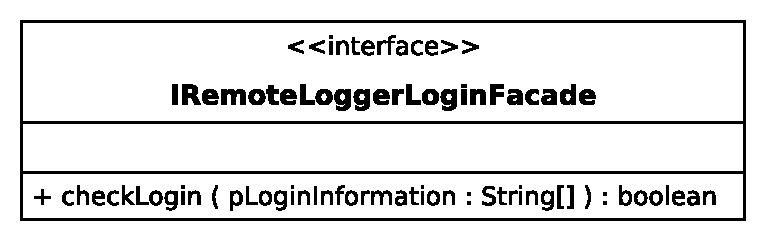
\includegraphics[width=180px]{../img/CD-IRemoteLoggerLoginFacade.eps}
	\caption{Aufbau der \glqq LoginFacade\grqq}
\end{wrapfigure}
\par Dieses Interface kapselt einen Teil des ADITO4-Benutzer-Frameworks (siehe \prettyref{fig:KommunikationServerManager}) für den Remote-Logger-Server. Dadurch lassen sich die vom Remote-Logger-Client erhaltenen Logininformationen (siehe \prettyref{fig:KommunikationServerManager}, Schritt 3) auf Gültigkeit prüfen.
\vspace{5px}
\par Um einen Loginversuch zu validieren, übergibt man der im Interface definierten Methode \glqq checkLogin(...)\grqq\ die zu prüfenden Informationen und man erhält als Rückgabewert, ob diese gültig sind. \\
\begin{figure}[htp] 
    \centering
	\begin{spacing}{0.75}
		\begin{javacode}[firstnumber=25]
@Override
public boolean checkLogin(@NotNull String[] pLoginInformation)
{
  ManagerLoginUtil.LoginResult result = ManagerLoginUtil.checkLogin(pLoginInformation, 
                                         securityPrefs, loginPrefs, locale, userDirectory);
  
  // Überprüft gleichzeitig, ob der hinter den Login-Informationen liegende Benutzer
  // die passende Rolle besitzt.
  return result.wasOK() && UserUtility.hasRole(result.getUser(), InternalRoles.ADMIN);
} 		\end{javacode}
	\end{spacing}
	\caption{Implementierung der \glqq checkLogin(...)\grqq-Methode (siehe Anhang \prettyref{sec:CODE_RemoteLoggerLoginFacadeImpl})}
\end{figure}

\subsubsection{IRemoteLoggerConnectionHandler}
\begin{wrapfigure}[10]{r}[0cm]{225px}
	\hspace{5px}
	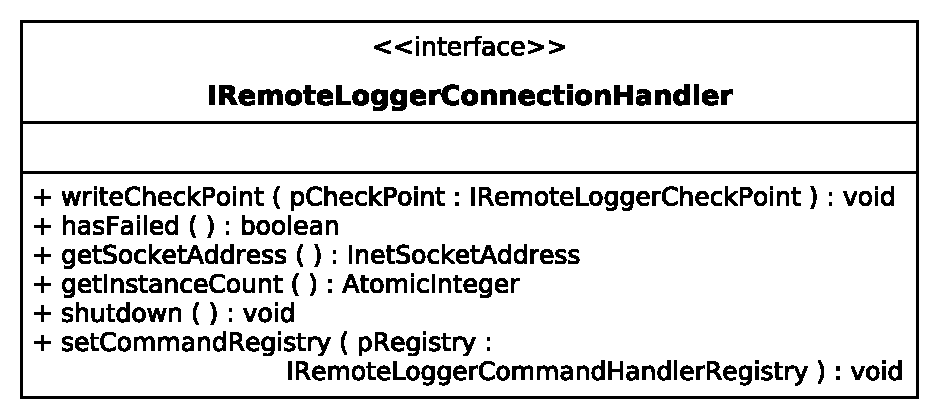
\includegraphics[width=220px]{../img/CD-IRemoteLoggerConnectionHandler.eps}
	\caption{Aufbau des \glqq IRemoteLoggerConnectionHandler\grqq}
\end{wrapfigure}
\par Der in Punkt \prettyref{sec:RemoteLogger} erwähnte \glqq Connection-Handler\grqq\, spezifiziert durch das Interface \glqq IRemoteLoggerConnectionHandler\grqq\ und implementiert in der Klasse \glqq RemoteLoggerServerConnectionHandler\grqq\, erhält mit der Methode \glqq writeCheckPoint(...)\grqq\ die Anweisung, einen IRemoteLoggerCheckPoint (\prettyref{sec:IRemoteLoggerCheckPoint}) an alle derzeit verbundenen und autorisierten Remote-Logger-Clients zu senden. Ebenso besitzt er die Aufgabe, eingehende Verbindungsanfragen von neuen Clients zu verarbeiten und zu speichern.
\par Beide Aufgaben sind getrennt implementiert: \\
Auf der einen Seite wird jeder im ADITO4-System aufgetretene CheckPoint an alle autorisierten Verbindung innerhalb der o.g. Verbindungsliste gesendet.\\
Auf der anderen Seite läuft ein isolierter Hintergrundprozess (siehe Anhang \prettyref{sec:CODE_RemoteLoggerConnectionHandler}), der auf die Verbindung eines Remote-Logger-Clients wartet. Diese Verbindungsanfrage wird in Zusammenarbeit mit einem \glqq Selector\grqq\ abgearbeitet und in eine \glqq IRemoteLoggerServerConnection\grqq\ gekapselt. Das resultierende Verbindungsobjekt wird in der Verbindungsliste abgelegt.
\par Wenn man nun beide Aufgaben kombiniert betrachtet fällt auf, dass diese asynchron ablaufen müssen. Beispielsweise könnte sich ein Remote-Logger-Client verbinden, während der \glqq Connection-Handler\grqq\ CheckPoints an alle ihm bekannten Verbindungen nach außen sendet. \\
Hier kommt das Java-Schlüsselwort \textbf{synchronized} zum Einsatz. Dies bewirkt, dass keine konkurrierenden Zugriffe auf das gleiche Objekt gemacht werden können, sondern anfallende Zugriffe sequentiell abgearbeitet werden müssen. Dadurch kann sichergestellt werden, dass die o.g. Verbindungsliste während dem Senden der Meldungen nicht manipuliert wird.

\subsubsection{IRemoteLoggerServerConnection}
\begin{wrapfigure}[9]{r}[0cm]{235px}
	\vspace{-10px} \hspace{5px}
	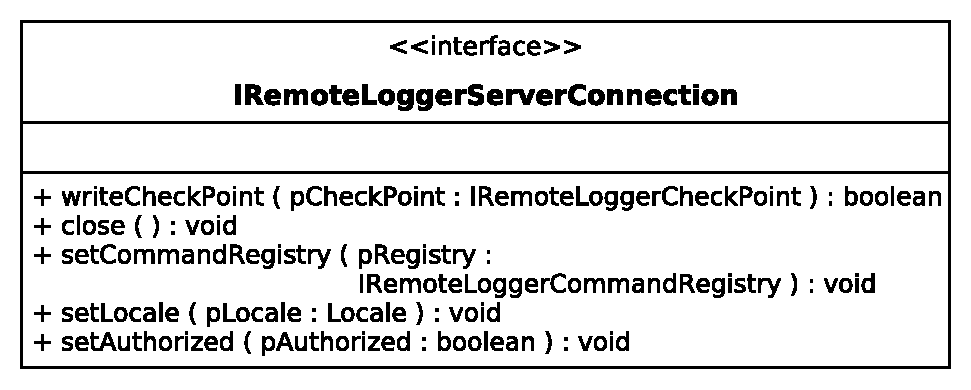
\includegraphics[width=230px]{../img/CD-IRemoteLoggerServerConnection.eps}
	\caption{Aufbau des Interfaces \glqq IRemoteLoggerServerConnection\grqq}
\end{wrapfigure}
\par Die Verbindung zwischen einem Remote-Logger-Server und Remote-Logger-Client wird hier repräsentiert. Diese Klasse ermöglicht es unter anderem, einen IRemoteLoggerCheckPoint in der für den jeweiligen Client passenden Sprache zu senden. Dieses Senden darf allerdings nur erfolgen, wenn die Verbindung davor durch ein IRemoteLoggerCommand autorisiert wurde (siehe \prettyref{sec:IRemoteLoggerCommand}). 
\par Ebenso werden hier etwaige empfangene Remote-Logger-Kommandos interpretiert und die zugehörigen \glqq IRemoteLoggerCommandHandler\grqq\ ausgeführt. Diese Kommunikationsschnittstelle zwischen Remote-Logger-Client und Remote-Logger-Server ist durch den in Punkt \prettyref{sec:ObjectInputStreamConsumer} angesprochenen ObjectInputStreamConsumer realisiert:
\begin{figure}[h] 
    \centering
	\begin{spacing}{0.75}
		\begin{javacode}[firstnumber=23]
  ObjectInputStreamConsumer.consume(Channels.newInputStream(pChannel), null, 
                                      this::_handleCommand, this::_handleException);\end{javacode}
	\end{spacing}
	\caption{ObjectInputStreamConsumer filtert den InputStream nach IRemoteLoggerCommands}
\end{figure}
\par Das Senden von IRemoteLoggerCheckPoints innerhalb der Methode \glqq writeCheckPoint(...)\grqq\ ist in der zugehörigen Implementierung durch einen ObjectOutputStream realisiert :
\begin{figure}[h] 
    \centering
	\begin{spacing}{0.75}
		\begin{javacode}[firstnumber=45]
ByteArrayOutputStream baos = new ByteArrayOutputStream();
ObjectOutputStream oos = new ObjectOutputStream(baos);
oos.writeObject(pCheckpoint);
oos.flush();

channel.write(ByteBuffer.wrap(baos.toByteArray()));\end{javacode}
	\end{spacing}
	\caption{Implementierung des Sendens von CheckPoints mittels einem ObjectOutputStream}
\end{figure}

\subsubsection{IRemoteLoggerCommandHandlerRegistry}
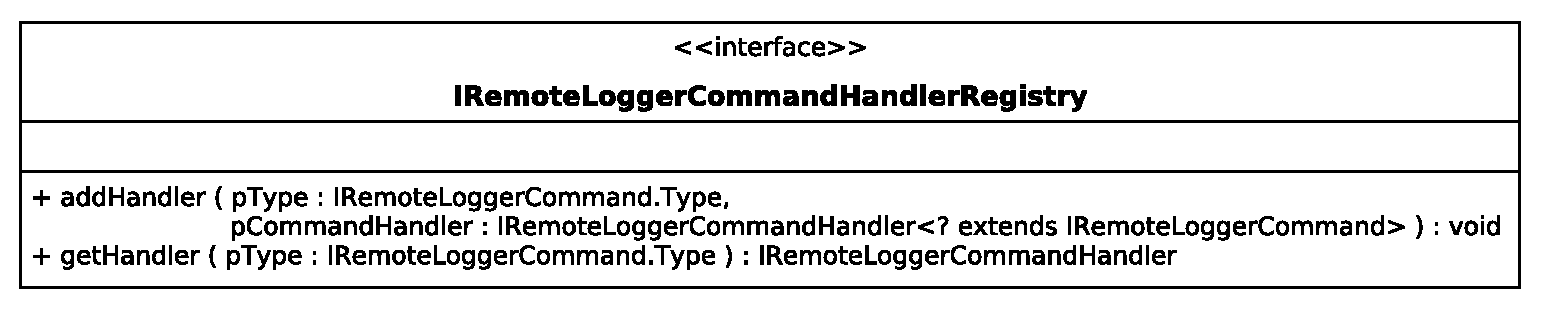
\includegraphics[width=\textwidth]{../img/CD-IRemoteLoggerCommandHandlerRegistry.eps}
\par In dieser Klasse lassen sich IRemoteLoggerCommandHandler mit ihren zugehörigen IRemoteLoggerCommands verknüpfen. Falls ein spezifischer CommandHandler für das Abarbeiten von IRemoteLoggerCommands benötigt wird, kann man diesen mit der getHandler(...)-Methode ermitteln.

\subsubsection{IRemoteLoggerCommandHandler}
\begin{wrapfigure}[7]{r}[0cm]{225px}
	\vspace{-20px} \hspace{5px}
	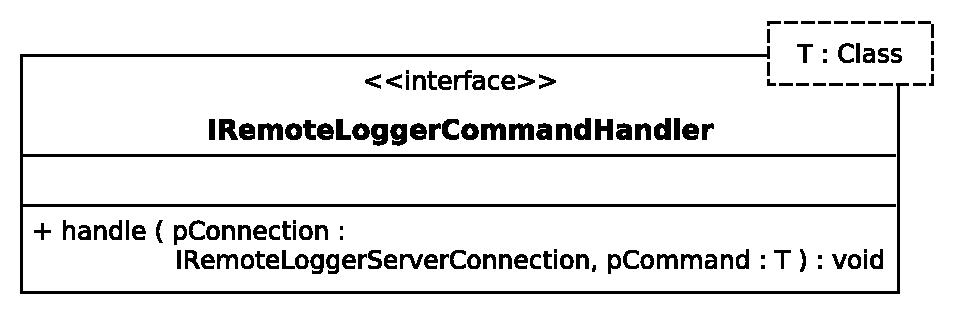
\includegraphics[width=220px]{../img/CD-IRemoteLoggerCommandHandler.eps}
	\caption{Aufbau des Interfaces \glqq IRemoteLoggerCommandHandler\grqq}
\end{wrapfigure}
\par Verarbeitet ein IRemoteLoggerCommand (\prettyref{sec:IRemoteLoggerCommand}), das vom Remote-Logger-Client zum Remote-Logger-Server gesendet wurde. Der Handler erhält hierzu über die \glqq handle(...)\grqq-Methode die IRemoteLoggerServerConnection, über die das Kommando empfangen wurde, und die Instanz des empfangenen Kommandos.
\par Als Beispiel für einen CommandHandler ist der \glqq AuthorizationCommandHandler\grqq\ (siehe Anhang \prettyref{sec:CODE_IRemoteLoggerCommand}) zu nennen. Diesem wird im Konstruktor die in Punkt \prettyref{sec:IRemoteLoggerLoginFacade} erwähnte Login-Facade übergeben, um die empfangenen Login-Informationen auf Richtigkeit zu prüfen. Wenn der Login gültig ist, wird die Verbindungsinstanz als autorisiert gekennzeichnet, andernfalls wird die Verbindung sofort geschlossen.
\begin{figure}[h] 
    \centering
	\begin{spacing}{0.75}
		\begin{javacode}[firstnumber=28]
@Override
public void handle(IRemoteLoggerServerConnection pConnection, AuthorizationCommand pCommand)
{
  IRemoteLoggerLoginFacade loginFacade = null;
  if(loginFacadeSupplier != null)
    loginFacade = loginFacadeSupplier.get();
    
  if (loginFacade == null || loginFacade.checkLogin(pCommand.getLoginInformation()))
    pConnection.setAuthorized(true);
  else
    pConnection.close();
}\end{javacode}
	\end{spacing}
	\caption{\glqq handle(...)\grqq-Methode des \glqq AuthorizationCommandHandlers\grqq}
\end{figure}